% Chapter 1
\stepcounter{cap}
%\chapter{cap1}
\label{cap5}

\mychapter{5}{Capitolul \arabic{cap} \\ MANAGEMENTUL ERORILOR}
%\chapter{\arabic{cap}.Introducere} % Main chapter title

\label{Chapter5} % For referencing the chapter elsewhere, use \ref{Chapter1} 

\thispagestyle{fancy}

%-----------------------------------------------------------------

\section{Tipuri de erori} 
\begin{itemize}
 \setlength\itemsep{0em}
	\item Erori de secvenţă
	\item Erori apărute la accesarea bazei de date
	\item Bază de date coruptă
\end{itemize}


\section{Detectarea erorilor}
Erorile sunt raportate pentru fiecare apel către şi dinspre interfaţa modului de predicţie. Toate funcţiile returnează un număr ce corespunde unui tip de eroare.

	\subsection{Erori de secvenţă}
	O maşină de stare va verifica încălcarea ordinii secvenţelor.
	
	\subsection{Erori la accesarea bazei de date}
	Trebuie evaluate rezultatele funcţiilor native de accesare ale bazei de date.

	\subsection{Bază de date coruptă}
	Trebuie evaluate rezultatele funcţiilor native de accesare ale bazei de date.

\begin{figure}[h!]
  \centering
   \centering{%
   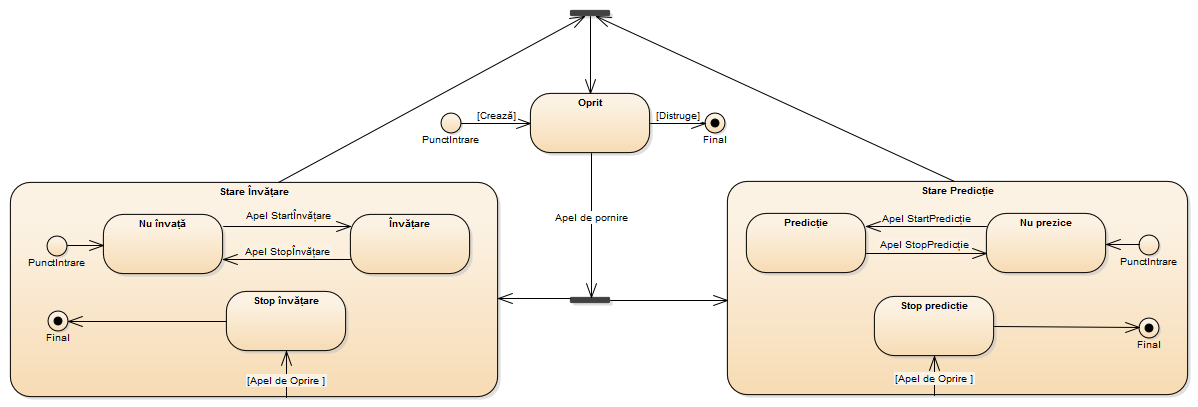
\includegraphics[width=0.8\textwidth]{Figures/masina_stare.png}}
  \caption{Mașină de stare pentru mecanismul învățare-predicție}
  \end{figure}		
	
\section{Tratarea erorilor}
În funcţie de tipul de eroare, aceasta poate fi prevenită pe viitor sau nu de către dezvoltator.
\vspace{6pt}
\\Există erori de secvenţă precum ``Înainte de apelarea funcţiei X este necesară pornirea unităţii software PNavPredictor''. Se poate întâmpla de asemenea ca atunci când dezvoltatorul porneşte procesul de predicţie de două ori consecutiv sa fie întâmpinat de eroarea ``Procesul de predicţie se află deja în curs de rulare''.
În astfel de cazuri este clar cum se pot preveni erorile.
\vspace{6pt}
\\Mai sunt însă şi cazuri ce nu pot fi tratate de către dezvoltator. Astfel de erori sunt cele precum ``Baza de date este coruptă'', ce pot să apară în cazul în care fişierul de sistem folosit pentru stocarea datelor este corupt. În aceste situaţii datele stocate anterior nu mai pot fi recuperate, toate informaţiile referitoare la rute fiind definitiv pierdute.



